\documentclass{article} % For LaTeX2e
\usepackage{wmw2026_conference,times}

% Optional math commands from https://github.com/goodfeli/dlbook_notation.
\input{math_commands.tex}

\usepackage{hyperref}
\usepackage{url}
\usepackage{graphicx}
\usepackage{amsmath}
\usepackage{booktabs}
\usepackage{xcolor}
\usepackage{float}

% Reduce spacing around figures and tables
\setlength{\textfloatsep}{8pt plus 1pt minus 1pt}
\setlength{\intextsep}{8pt plus 1pt minus 1pt}
\setlength{\abovecaptionskip}{4pt}
\setlength{\belowcaptionskip}{4pt}

\title{Self-Supervised Multi-Modal World Model with 4D Space-Time Embedding}

\author{Lance Legel\thanks{Correspondence: \texttt{lance@ecodash.ai}} \\
Ecological Intelligence Lab \\
Ecodash.ai \\
\AND
Qin Huang \\
School of Complex Adaptive Systems \\
Arizona State University \\
\And
Brandon Voelker \\
Geosensing Systems Engineering \& Sciences Lab \\
University of Houston \\
\AND
Daniel Neamati \\
Navigation \& Autonomous Vehicles Lab \\
Stanford University \\
\And
Patrick Alan Johnson \\
Earth System Lab \\
Allen Institute for Artificial Intelligence \\
\AND
Favyen Bastani \\
Earth System Lab \\
Allen Institute for Artificial Intelligence \\
\And
Jeff Rose \\
Spatial Intelligence Lab \\
SpatialLogic.com \\
\AND
James Ryan Hennessy \\
Department of Computer Science \\
Georgia Tech Institute of Technology \\
\And
Robert Guralnick \\
Florida Museum of Natural History \\
University of Florida \\
\AND
Douglas Soltis \\
Florida Museum of Natural History \\
University of Florida \\
\And
Pamela Soltis \\
Florida Museum of Natural History \\
University of Florida \\
\AND
Shaowen Wang \\
NSF Institute for Geospatial Understanding \\
University of Illinois Urbana-Champaign \\
}

\wmwfinalcopy % Uncomment for camera-ready version, but NOT for submission.

\begin{document}

\maketitle

\begin{abstract}
We present \textit{DeepEarth}, a self-supervised multi-modal world model with \textit{Earth4D}, a novel planetary-scale 4D space-time positional encoder. Earth4D extends 3D multi-resolution hash encoding to include time, efficiently scaling across the planet over centuries with sub-meter, sub-second precision. Multi-modal encoders (\textit{e.g.} vision-language models) are fused with Earth4D embeddings and trained via masked reconstruction. We demonstrate Earth4D's expressive power by achieving state-of-the-art performance on an ecological forecasting benchmark. Earth4D with learnable hash probing surpasses a multi-modal foundation model pre-trained on substantially more data. Access open source code and download models at: \\
\url{https://github.com/legel/deepearth}.
\end{abstract}

\section{DeepEarth Architecture}
\label{sec:deepearth_architecture}

DeepEarth is a self-supervised multi-modal world model that learns unified representations of Earth observation data across space and time. As seen in Figure~\ref{fig:inductive_simulator}, the architecture processes multi-modal inputs (\textit{e.g.} vision, language, sensor data) sampled around spatio-temporal events. The Earth4D encoder maps continuous space-time coordinates (\textit{latitude}, \textit{longitude}, \textit{elevation}, \textit{time}) to learnable positional embeddings, which are fused with embeddings from modality-specific encoders and processed as tokens in an autoencoder context window. Inspired by PerceiverIO \citep{Jaegle2021PerceiverIA}, V-JEPA 2 \citep{assran2025vjepa2selfsupervisedvideo}, Galileo \citep{tsenggalileo}, and AlphaEarth \citep{brown2025alphaearthfoundationsembeddingfield}, DeepEarth learns to generatively reconstruct and simulate joint distributions of multi-modal data.

\begin{figure}[H]
\centering
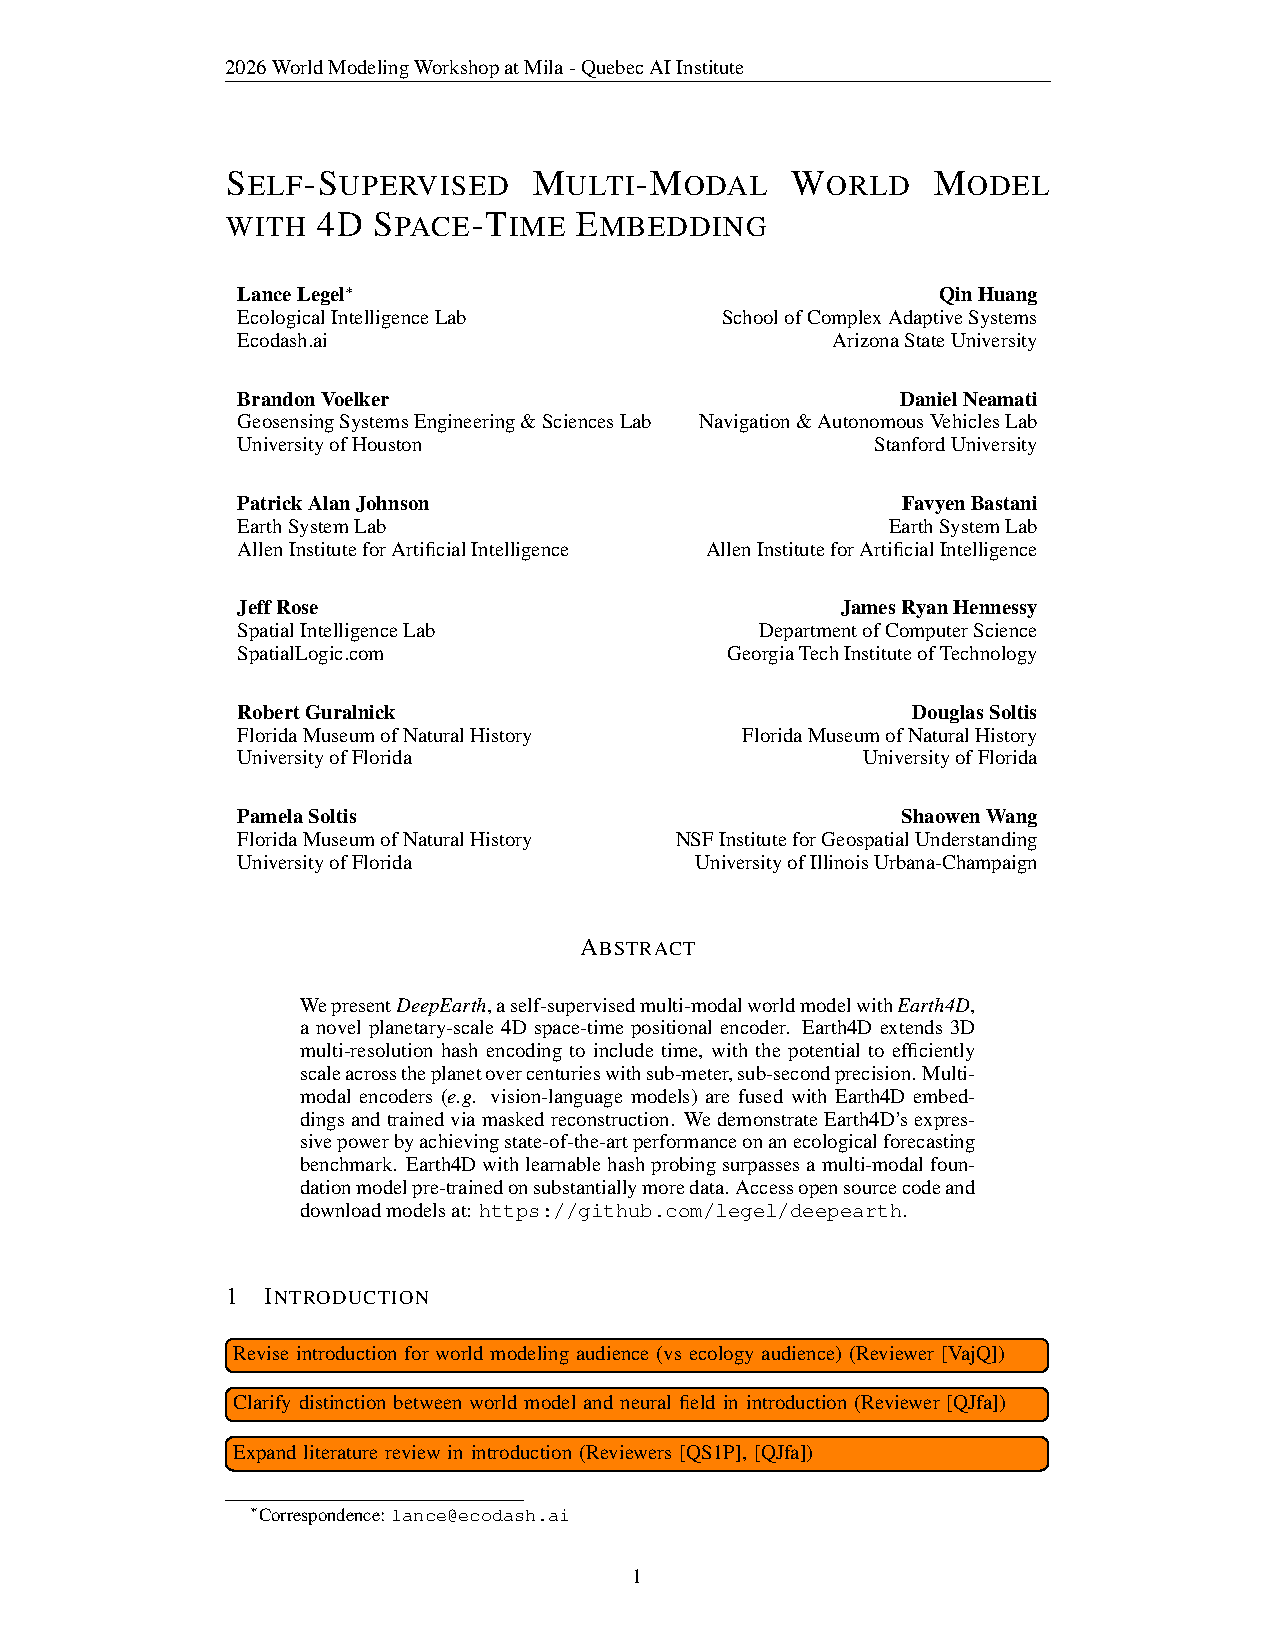
\includegraphics[width=\textwidth]{figures/deepearth.pdf}
\caption{\textbf{DeepEarth Overview.} Masked multi-modal data (\textit{e.g.} images, text) sampled around an event (\textit{e.g.} pollination) are encoded and fused with Earth4D space-time embeddings. These universal tokens are jointly encoded, and then masked data is inductively decoded and simulated.}
\label{fig:inductive_simulator}
\end{figure}

\section{Earth4D Architecture}
\label{sec:earth4d_architecture}

Following Grid4D \citep{xu2024grid4d}, Earth4D extends NVIDIA's multi-resolution hash encoding \citep{M_ller_2022} to four dimensions (Figure~\ref{fig:earth4d_encoder}) by concatenating features from one spatial (\textit{xyz}) and three spatio-temporal (\textit{xyt}, \textit{yzt}, \textit{xzt}) grids. Implemented as a standalone PyTorch module with massively parallelizable CUDA kernels, Earth4D is suitable for integration into larger models.

\begin{figure}[H]
  \centering
  \includegraphics[width=\textwidth]{figures/earth4d.pdf}
  \caption{\textbf{Earth4D Space-Time Positional Encoding.} A planetary-scale 4D encoder with fully decomposable spatio-temporal representation. Four grids (\textit{xyz}, \textit{xyt}, \textit{yzt}, \textit{xzt}) are each learned in 3D space and computed in parallel. Each grid has multiple resolution levels (Appendix~\ref{appendix:resolution}), enabling deep learning of complex joint distributions in multi-modal data across space-time scales.
}
  \label{fig:earth4d_encoder}
\end{figure}

Earth4D's hash encoding compresses spatial features into a fixed memory budget, but different coordinates can map to the same memory location (collisions). We integrate learned hash probing \citep{takikawa2023compactneuralgraphicsprimitives}, an end-to-end differentiable system that learns optimal memory allocation patterns for the data. This yields substantial performance improvements across tasks (Appendix~\ref{appendix:learned_probing}).

\section{Earth4D Experimental Validation}
\label{sec:experiments}

\subsection{Live Fuel Moisture Content Prediction}

\noindent\textbf{\textit{Dataset.}} Live Fuel Moisture Content (LFMC) measures the percentage of water in vegetation relative to its dry weight, a critical indicator for wildfire risk assessment. We evaluate Earth4D on Globe-LFMC 2.0 \citep{yebra2024globe}, a global ecological forecasting benchmark containing field measurements across diverse plant species, geographic regions, and temporal periods.

\noindent\textbf{\textit{Baseline Model.}} We compare against Galileo \citep{johnson2025highresolutionlivefuelmoisture,tsenggalileo}, a pre-trained Vision Transformer processing multi-modal remote sensing data (Appendix~\ref{appendix:benchmark}).

\noindent\textbf{\textit{Architecture.}} Earth4D encodes (\textit{x,y,z,t}) into a 192D vector, concatenated with a learnable species embedding initialized randomly (no prior knowledge). An MLP then predicts LFMC \%.

\begin{figure}[t]
\centering
\includegraphics[width=\textwidth]{figures/error_distribution_histogram.png}
\includegraphics[width=\textwidth]{figures/geospatial_temporal_test.png}
\caption{\textbf{Earth4D LFMC Prediction Performance.} \textit{(Top)} Distribution of absolute errors in percentage point predictions across 13,297 test samples, showing median error of 7.1pp. \textit{(A)} Geographic error distribution across CONUS shows low error in well-sampled regions. \textit{(B)} Temporal predictions closely track ground truth LFMC measurements across seasons (2017--2023).}
\label{fig:error_dist}
\end{figure}

\noindent\textbf{\textit{Results.}} Earth4D achieves MAE 12.1pp and R² 0.755, surpassing Galileo (MAE 12.6pp, R² 0.72) using only (\textit{x,y,z,t}) coordinates and species embeddings (Table~\ref{tab:lfmc_results}).

\begin{table}[h]
\centering
\small
\begin{tabular}{@{}llccc@{}}
\toprule
\textbf{Model} & \textbf{Data Inputs} & \textbf{MAE (pp)} & \textbf{RMSE (pp)} & \textbf{R²} \\
\midrule
\textbf{\textit{Galileo}} (Pre-Trained) & (\textit{x,y,z,t}) + Species Type + Remote Sensing & 12.6 & \textbf{18.9} & 0.72 \\
\textbf{\textit{Earth4D}} (Learned Hashing) & (\textit{x,y,z,t}) + Species Name & \textbf{12.1} & 19.9 & \textbf{0.755} \\
\bottomrule
\end{tabular}
\caption{\textbf{State-of-the-Art Ecological Forecasting Benchmark.} Earth4D surpasses the pre-trained Galileo foundation model without satellite imagery, weather data, or topography.}
\label{tab:lfmc_results}
\end{table}

\subsection{RGB Aerial Imagery Reconstruction}

We evaluate Earth4D's ability to infer RGB pixels from (\textit{x,y,z,t}) inputs with objective (\textit{x,y,z,t}) $\rightarrow$ (\textit{r,g,b}). Using USGS 3DEP LiDAR \citep{stoker2022accuracy,sugarbaker20143d} and USDA NAIP imagery \citep{USDA_NAIP} paired by \citet{allred2025canopy}, we train on 5.8M coordinate-color pairs from Houston coastal wetlands (Figure~\ref{fig:rgb_reconstruction}).

\begin{figure}[H]
\centering
\includegraphics[width=\textwidth]{figures/rgb_reconstruction.png}
\caption{\textbf{RGB Reconstruction from LiDAR Elevation.} Houston coastal wetlands, 2018. \textit{Left to right:} LiDAR height, ground truth, baseline, learned probing (18\% lower loss).}
\label{fig:rgb_reconstruction}
\end{figure}

\newpage

\bibliography{deepearth}
\bibliographystyle{wmw2026_conference}

\newpage

\appendix

\section*{APPENDICES}
\addcontentsline{toc}{section}{Appendices}

\section{Earth4D Resolution Specifications}
\label{appendix:resolution}

\begin{figure}[H]
\centering
\includegraphics[width=\textwidth]{figures/earth4d_resolution_levels.png}
\caption{\textbf{Earth4D Space-Time Scales.} Default 24$\times$24$\times$24 levels for each \textit{xyz}, \textit{xyt}, \textit{yzt}, \textit{xzt} grid. Each level stores up to $2^{22}$ entries, with each entry storing a 2D feature. Requires 724M trainable parameters ($\sim$11 GB GPU memory during training). Parallelizable across levels and spatio-temporal boundaries. Outputs 192D per $(x,y,z,t)$ coordinate from 4 grids $\times$ 24 levels $\times$ 2D feature per level. Hashing saves memory vs.\ naive requirement, e.g., $(2^{28})^3 = 10^{25}$ at level 24.}
\label{fig:earth4d_specs}
\end{figure}

\newpage

\section{Learned Hash Probing and Ablation Studies}
\label{appendix:learned_probing}

\subsection{Hash Collision Simulations}
\label{appendix:collisions}

\begin{figure}[H]
\centering
\footnotesize
\setlength{\tabcolsep}{4pt}
\begin{tabular}{@{}llll@{}}
\toprule
\textbf{Scenario} & \textbf{Spatial} & \textbf{Temporal} & \textbf{Description} \\
\midrule
\textit{Uniform Random} & Global & Full & Uniform Earth surface sampling \\
\textit{Continental Sparse} & North America & Full & Sparse continental coverage \\
\textit{Moderate Spatial Cluster} & 10km $\times$ 10km & Full & City-scale clustering \\
\textit{Moderate Temporal Cluster} & 1k locations & Distributed & Temporal sampling at fixed locations \\
\textit{Moderate Spatiotemporal} & 1km $\times$ 1km & 1 hour & Neighborhood-scale event \\
\textit{Extreme Spatial Single} & 10m $\times$ 10m & Full & Building-scale dense clustering \\
\textit{Extreme Spatial Multi} & 10 $\times$ (10m $\times$ 10m) & Full & 10 dense clusters worldwide \\
\textit{Extreme Temporal Single} & Global & 1 hour & Global snapshot \\
\textit{Extreme Temporal Multi} & Global & 10 $\times$ (1 hour) & 10 temporal snapshots \\
\textit{Time Series} & 10k locations & 100 steps & Regular temporal sampling \\
\bottomrule
\end{tabular}

\vspace{0.5em}

\includegraphics[width=\textwidth]{figures/1M_hash_collision_rate.png}
\caption{\textbf{Earth4D Hash Collision Analysis.} \textit{(Table)} 10 $(x,y,z,t)$ point distribution scenarios that were simulated to analyze hash collisions in Earth4D memory. \textit{(Graph)} Shows results for 1M point simulations across all 24 levels.}
\label{fig:collision_rates}
\end{figure}

\subsection{Performance Improvements}
\label{appendix:baseline_results}

Standard multi-resolution hash encoding without learned probing obtains RMSE 26.0pp, MAE 16.6pp, and R² 0.58 (800M parameters, $2^{22}$ hash capacity). Integrating learned hash probing \citep{takikawa2023compactneuralgraphicsprimitives}, which learns to select optimal hash table indices from a candidate set, yields RMSE 19.9pp, MAE 12.1pp, and R² 0.755—a 27.1\% MAE reduction and 30.2\% R² improvement. Extreme compression to 5M parameters (99.3\% reduction, $2^{14}$ hash capacity) achieves MAE 15.0pp/R² 0.668, outperforming the 800M baseline by 14.7\% in R² with 4$\times$ training speedup and 93\% memory reduction. On RGB reconstruction, learned probing reduces validation loss by 18\%. These gains result from collision reduction (33\% at 1M points) and learned shared features across memory indices, allowing the model to discover meaningful spatio-temporal patterns.

\newpage

\section{Benchmark Specifications}
\label{appendix:benchmark}

\subsection{Galileo Baseline Model}

Galileo \citep{johnson2025highresolutionlivefuelmoisture,tsenggalileo} is a Vision Transformer \citep{dosovitskiy2021an} (5.3M parameters) pre-trained by the Allen Institute for AI. It processes Sentinel-2 optical imagery \citep{drusch2012sentinel}, Sentinel-1 SAR \citep{torres2012gmes}, VIIRS night lights, ERA-5 weather \citep{munozsabater2019era5}, TerraClimate soil/water data \citep{abatzoglou2018terraclimate}, SRTM topography \citep{farr2000shuttle}, (\textit{x,y,z,t}) coordinates, and species type. We use the Allen Institute for AI's exact Globe-LFMC 2.0 \citep{yebra2024globe} train/test split (76,467/13,297) to directly compare against this benchmark.

\end{document}
